\section{Understanding Kiva website and Dataset}

\begin{itemize}
	\item Describe what user can do on the website: search for Projects, Auto-lending setup
	\item Describe how to get the data using GraphQL, Crawling method
	\item Describe data schema: fields that we can get, the meaning of each fields
	\item Describe preprocessing steps with the data
	      \begin{itemize}
		      \item Steps: accelerated loading, forming the big table, removing unwanted tags, remove anonymous Lenders, handle duplicates\dots
		      \item Forming the tri-partite graph: Lenders-Projects-Tags
		      \item Mention that we have to use CuDF for accelerated data handling
	      \end{itemize}
\end{itemize}

In this section, we will describe the Kiva website and the dataset that we use in this thesis.
We will also describe the preprocessing steps that we have to do with the dataset.

While there are many crowdfunding platforms,
we specifically choose Kiva because of its transparancy and the avalability of the data for public access.

\subsection{Kiva website}

To understand the data that the platform provides, we have to understand the interface that the platform provides to its users.
Like other platform, Kiva has a website where users can login and interact with the platform.
To understand the data that the platform provides and to extract meaningfull insight from the data,
we have to understand the interface that the platform provides to its users.

Any website interface is designed to make users interact with it in a pre-defined way.
In Kiva, we belived that the most function that users can do is to search for projects that they want to fund.
Or they can setup an Auto-Lending program, which will automatically fund projects that fit their criteria.


\begin{figure}[H]
	\centering
	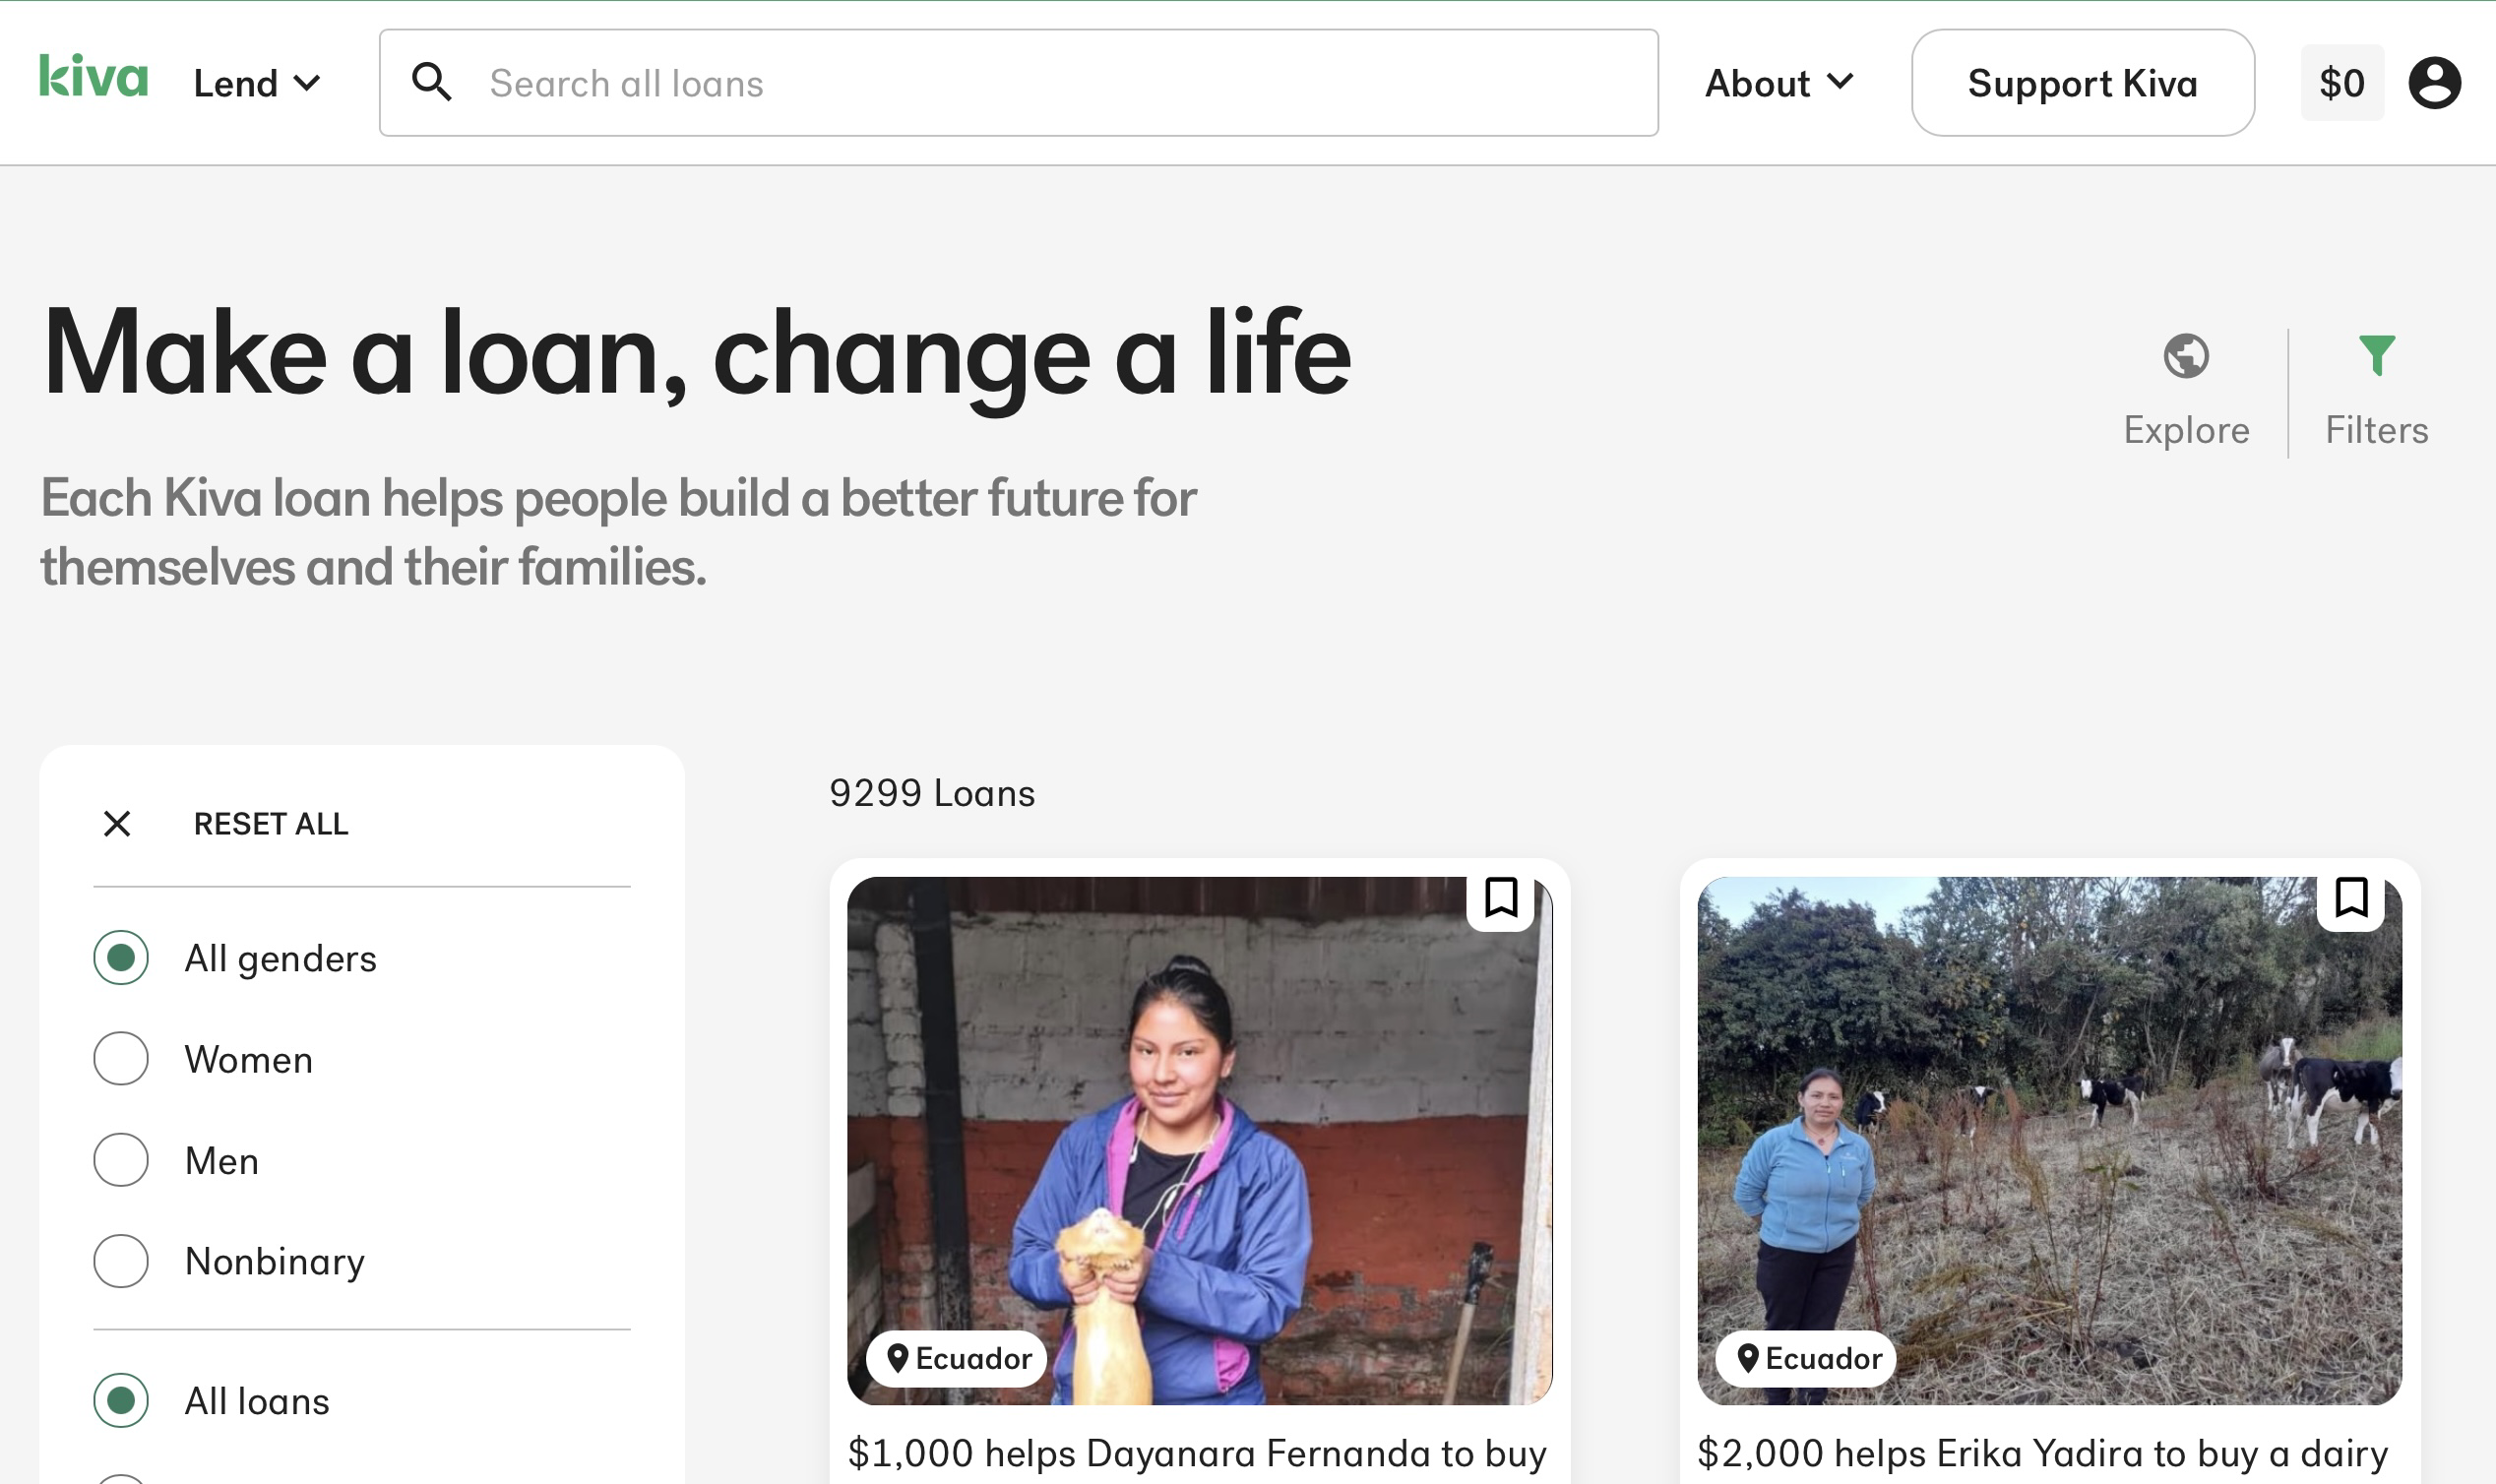
\includegraphics[width=0.8\textwidth]{images/kiva-browse-project.png}
	\caption{Kiva website interface for browsing projects}
	\label{fig:kiva-browser-project}
\end{figure}

It is important to know what Lenders can do when looking for his or her interested project.

Some criteria that they could do is

\begin{table}[H]
	\centering
	\begin{tabular}{|c|c|c|c|}
		\hline
		   & Meaning                       & Type            & choices                                                                                                                 \\
		\hline
		1  & Gender of the borrower button & Choice          & Woman or Men or Nonbinary                                                                                               \\
		2  & Filter by type of Loan        & Choice          & Individual or Group                                                                                                     \\
		3  & Search by keyword             & Text            & Put any keyword to search in the stories of Projects                                                                    \\
		4  & Sort Order                    & Choice          & Amount: High to Low, Amount left, Amount: Low to High, Ending soon, Most recent, Trending now, Loan Length, Recommended \\
		5  & Location                      & Multiple choice & Choose from a list of countries                                                                                         \\
		6  & Sector                        & Multiple choice & Choose from a list of sectors                                                                                           \\
		7  & Attribute                     & Multiple choice & Choose from a list of attributes                                                                                        \\
		8  & Tags                          & Multiple choice & Choose from a list of tags                                                                                              \\
		9  & Loan Length                   & Choice          & All loans, 8 month or less, 16 months or less, 2 years or less, 2 years or more                                         \\
		10 & Loan Distribution             & Choice          & All loans, Parter, Direct                                                                                               \\
		11 & Partner Info                  & Text            & Search by Parter name                                                                                                   \\
		12 & Risk Rateing                  & Range           & From 1 to 5                                                                                                             \\
		13 & Default Rate                  & Range           & From 0\% to 100\%                                                                                                       \\
		14 & Profitability                 & Range           & From -160\% to 90\%                                                                                                     \\
		\hline
	\end{tabular}
	\caption{Table with 4 columns}
	\label{tab:mytable}
\end{table}






\section{Basic data statistics}

\begin{itemize}
	\item Worldwide statistics
	      \begin{itemize}
		      \item How many projects
		      \item how many lenders
		      \item projects vs country distribution
		      \item successful rate
		      \item \textbf{How long that users stay on the platform}
	      \end{itemize}
	\item Vietnam statistics
	      \begin{itemize}
		      \item How many projects
		      \item \dots
	      \end{itemize}
\end{itemize}